\documentclass{article}

% use Times
\usepackage{times}
% For figures
\usepackage{graphicx} % more modern
%\usepackage{epsfig} % less modern
\usepackage{subfigure} 

% For citations
\usepackage{natbib}

% For algorithms
\usepackage{algorithm}
\usepackage{algorithmic}

% As of 2011, we use the hyperref package to produce hyperlinks in the
% resulting PDF.  If this breaks your system, please commend out the
% following usepackage line and replace \usepackage{icml2014} with
% \usepackage[nohyperref]{icml2014} above.
\usepackage{hyperref}

% Packages hyperref and algorithmic misbehave sometimes.  We can fix
% this with the following command.
\newcommand{\theHalgorithm}{\arabic{algorithm}}

% Employ the following version of the ``usepackage'' statement for
% submitting the draft version of the paper for review.  This will set
% the note in the first column to ``Under review.  Do not distribute.''
\usepackage[accepted]{icml2014} 


% The \icmltitle you define below is probably too long as a header.
% Therefore, a short form for the running title is supplied here:
\icmltitlerunning{DIXON}

\begin{document} 

\twocolumn[
\icmltitle{Comp 562 Final Project\\Comparison of Machine Learning Methods for Analyzing Mental Health Data}

% It is OKAY to include author information, even for blind
% submissions: the style file will automatically remove it for you
% unless you've provided the [accepted] option to the icml2014
% package.
\icmlauthor{Elise Dixon}{PID: 730079241}

% You may provide any keywords that you 
% find helpful for describing your paper; these are used to populate 
% the "keywords" metadata in the PDF but will not be shown in the document
\icmlkeywords{boring formatting information, machine learning}

\vskip 0.3in
]

\begin{abstract} 
The rate of people around the world being diagnosed with mental health conditions continues to grow, making it one of the leading cause of disability world-wide. In this paper, the factors that may lead someone towards treatment by a mental health professional or not are examined. Employing five different machine learning algorithms, this project was able to reach an accuracy of 89\% with an eXtreme Gradient Boosting model. The other models had close results with a range of 85-87\% accuracy. Further iterations of this project could append the more recent datasets gathered.
\end{abstract} 


\section{Introduction}

\subsection{Motivation}

Mental health remains a highly prevalent concern for people worldwide, yet continues to be stigmatized and shied away from. The Canadian Mental Health Association released information noting that 1 in 4 people are affected by mental illness. However, it also noted that children with anxiety disorders are less likely to receive treatment. So while there are many resources available for people to get the care that they need, there is a disconnect. 

The goal of this project was to discover some of that factors that may dissuade a person from seeking professional treatment. With this, professionals in this field can see where resources may be lacking. Also, projects such as these will serve as a reminder of the tangible impact that technology can have outside of its own industry. It will spark more initiatives into how machine learning can help in the medical field. In the future, it can be used to develop treatment plans and potential predict crises. 

\subsection{Data}

A dataset gathered by Open Sourcing Mental Illness (OSMI) Ltd in 2016 was used, which includes over 1400 survey entries from across the world. It is known as the 'Mental Health in Tech' survey, which specifically targets those who work in the technology industry. This study has been done for the past 6 years, however, the 2016 dataset included the largest number of responses. The survey included about 40 questions related to a person's personal information (such as their gender identity and age) as well as work specific questions (such as if they received healthcare coverage specific to mental illness through their employer).

\section{Preprocessing} 

\subsection{Refactoring the Data}
 
Once initially looking at the data, it became clear that the data was crowded will large blocks of text that made it difficult to parse through. This required some refactoring, in which the column names were shortened from full questions to a few key words. It was also clear that some features would not be helpful to the model. This included fields that had fill in the blank responses rather than multiple course.Without additional algorithms like sentiment analysis, there would be no way to efficiently categorize that data. Because of this, these entries were cleaned from the dataset prior to being read in the Jupyter notebook.

After opening it into a pandas Dataframe, the sections of the data with mostly empty fields were removed. This reduced the dataset to ~960 entries. The last task within cleaning the data was to categorize the age and gender fields. The gender feature was filtered into three sections: {\tt male}, {\tt female}, and {\tt Genderqueer/Other}. Within the age feature, there were some anomalies, including an age of 3 and 323. These were all assigned the value of the {\tt mean\_age}: 34.  

\subsection{Exploratory Data Analysis}

After encoding and scaling the data, I began an exploratory data analysis. This included parsing the data in various ways and creating data visualizations in order to better understand the dataset. I was then able to find the 10 features most correlated with {\tt sought\_treatment}. This results of this analysis in the heatmap in Figure 1.

\begin{figure}
  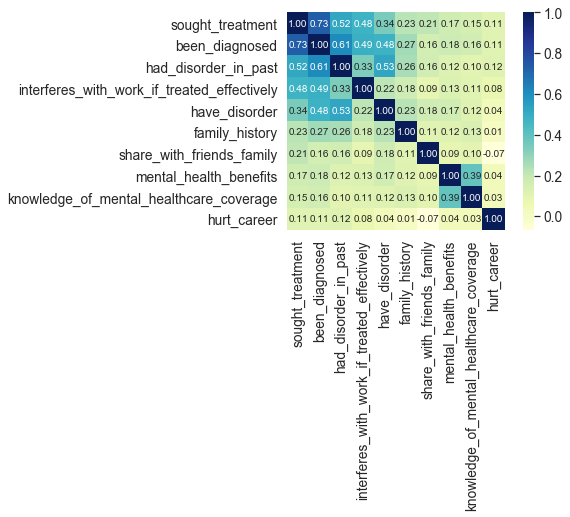
\includegraphics[width=\linewidth]{corrmat.png}
  \caption{Heatmap of features most correlated with sought\_treatment}
  \label{fig:corrmat}
\end{figure}
 I also looked at specific features in relation to one another and found that while men did report having a mental illness, none of them had sought treatment (shown in Figures 2 and 3). 
 \begin{figure}
  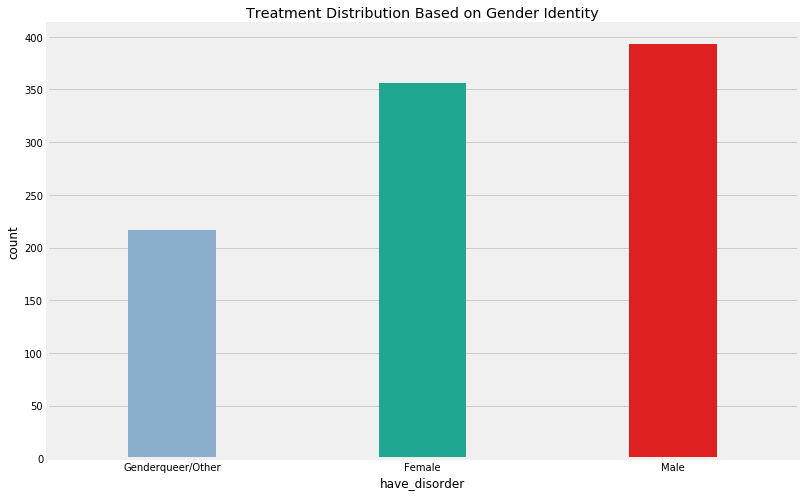
\includegraphics[width=\linewidth]{have_disorder.png}
  \caption{Mental Illness Distribution based on Gender Identity}
  \label{fig:have_disorder}
\end{figure}
\begin{figure}
  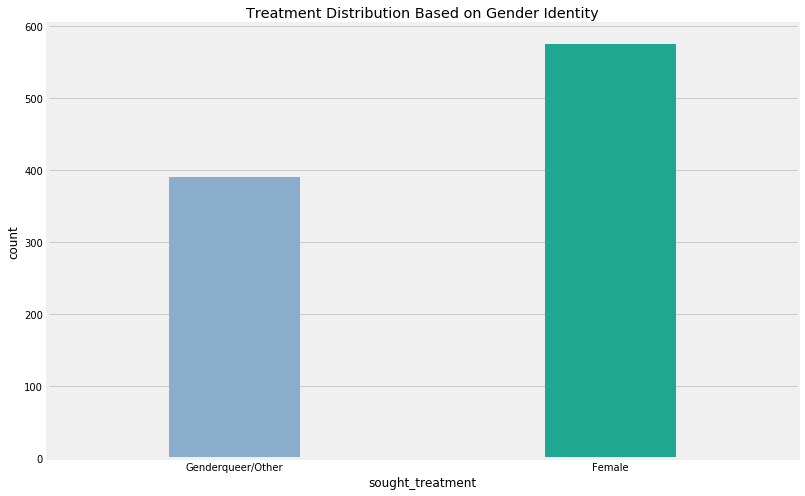
\includegraphics[width=\linewidth]{treatment.png}
  \caption{Treatment Distribution based on Gender Identity}
  \label{fig:treatment}
\end{figure}
\section{Modeling} 

\subsection{Random Forest Tree}
Known for its training speed, the Random Forest Tree is able to maintain accuracy with minimal run time. It uses a random sampling of data in order to better predict the target output. This model resulted in an accuracy of 87.1\%
\subsection{Logistic Regression}
A commonly used algorithm, logistic regression has an output that can be considered a probability. Due to its simplicity as far as interpretation and scalability, it was considered a good candidate for this analysis. It preformed on par with the Random Forest Tree with an average accuracy of 87.1\%
\subsection{Support Vector Machine(SVM)}
While SVMs tend to struggle with large datasets, their effectiveness with binary classification fit the problem well. The lack of speed computationally made it a less desirable choice, however the results were not affected by the nearly 1,000 entries. With an accuracy of 85.6\%, the SVM model performed the lowest of the five models, however it stayed with one standard deviation of the others. 
\subsection{Gaussian Naive Bayes}
The Gaussian Naive Bayes model is computationally fast and has ease with its implementation. However, it can have difficulty with predictions as it will result in a probability estimate of zero if a specific class label and attribute value are not paired. This often results in a low precision. With this dataset, it resulted in an accuracy of 86.6\%. 
\subsection{eXtreme Gradient Boosting(XGBoost)}
After completing the analysis of the previous four methods and finding similar results, both in terms of accuracy as well as AUC score, I decided to include the eXtreme Gradient Boosting Model. It is known for having both high perform and speed. Using the gradient boosting framework, XGBoost builds sequentially, improving upon previous models in order to minimize error. Additionally, the algorithm is high inter-operable, working on Mac, Windows and Linux, as well as commonly developed across programming languages and cloud platforms. The XGBoost model implemented outperformed the other four with an accuracy of 88.7\%.
\subsection{Results}
Overall, each of the models performed well with little variance between them. The differences found were marginal. However, there were definite distinctions in the performance values that were reported, as shown in Table 1. XBGoost significantly outperformed the other models in accuracy and performance metrics. 

\begin{table}[t]
\caption{Classification report of each machine learning model. Note: TPR = true positive rate, TNR = true negative rate, FPR = false positive rate, and FNR = false negative rate}
\label{sample-table}
\vskip 0.15in
\begin{center}
\begin{small}
\begin{sc}
\begin{tabular}{lcccr}
\hline
\abovespace\belowspace
Data set & TPR & TNR & FPR & FNR\\
\hline
\abovespace
R. Forest Tree    & .835 & .893  & .10. &.175 \\
L.Regression & .789& .919 &.081 &.021\\
SVM    & .737& .893 &.107&.175\\
Naive Bayes    & .794& .904 &.095 &.206       \\
XGBoost     & .854& .902 &.098 &.145\\
\belowspace
\end{tabular}
\end{sc}
\end{small}
\end{center}
\vskip -0.1in
\end{table}

\section{Summary}
\subsection{Conclusion} 
In this experiment, a number of supervised learning algorithms were compared in order determine which could most accurately predict whether a person would seek treatment given different life factors. Through this analysis, I was able to conclude that the most significant factors were whether the person had a disorder, which is a logical conclusion, or whether they had a family history of mental illness. Additionally, I found that XGBoost was well equipped to predict the outcome of this dataset.
\subsection{Future Work} 
In the future, I would hope to have a larger dataset and more entries that include male identifying persons who have sought treatment. Figure 2 alone demonstrations the stigma around gender identify and mental health. I hope to bring light to these issues and using real data is a great place to start.

\bibliography{main}
\bibliographystyle{icml2014}
\begin{enumerate}
	\item Abbas, N. M. (2019, September 5). Machine Learning and Mental Health. 
	\item Khondoker, M., Dobson, R., Skirrow, C., Simmons, A., & Stahl, D. (2016). A comparison of machine learning methods for classification using simulation with multiple real data examples from mental health studies. Statistical Methods in Medical Research, 25(5), 1804–1823. doi: 10.1177/096228021350243
	\item Morde, V. (2019, April 8). XGBoost Algorithm: Long May She Reign!
	\item Navlani, Avinash. Understanding Logistic Regression in Python. (2018, September 7). 
\end{enumerate}
\end{document} 